\section{04 - Wahrnehmung}

\subsection{Visuelle Wahrnehmung}

Palmer's 4-Stufen-Modell: Retinal Image (2D Projektion)
$\rightarrow$ Image (Bildatome, z.B. Kanten)
$\rightarrow$ Surfaces (Zusammengehörende Flächen)
$\rightarrow$ Objects (3D-Objekte, Tiefensinn)
$\rightarrow$ Categories (Einschätzung, Interpretation).

Die \textbf{Retina} ist die Netzhaut, und enthält Stäbchen und Zapfen als Sensorzellen
sowie davor Bipolar-, Amakrin-, Horizontal- und Ganglienzellen zur Verarbeitung
und Sammlung der Informationen und Weiterleitung über den Sehnerv.

Jede Ganglienzelle ist mit mehreren Sensorzellen verknüpft, der Bereich heißt
\textbf{Rezeptives Feld}. Die verschiedenenen rezeptiven Felder überlappen sich, die
Informationen werden also mehrfach verwendet.

Der Bereich mit der höchsten Zapfendichte heißt
\textbf{Fovea}, und hat etwa 0.5mm Durchmesser. In diesem Bereich sind keine anderen
Zellen den Sensorenzellen vorgelagert. Hier hat man optimale Schärfe, aber wegen
der Bauart kann nur ein kleiner Bereich so gestaltet sein. Daher muss man das
Auge bewegen, um die Umwelt wahrzunehmen.

\textbf{Zapfen} sind farbempfindlich (rot/grün/blau), und besonders scharf in der Mitte.
\textbf{Stäbchen} sind sehr lichtempfindlich, funktionieren also nicht bei starker
Helligkeit, dafür ermöglichen sie Nachtsehen. Sie sind mehr in der Peripherie angeordnet
als im Zentrum.

Der Sehwinkel des Menschen beträgt etwa $1^\circ$. Dies entspricht einer Länge von 12pt bei
einem Abstand von 30cm. Die Darstellungsgröße, etwa von Schrift, muss daher auf das
Medium angepasst werden. Je weiter weg von der Fovea, desto größer muss etwas dargestellt
werden, um erkennbar zu sein.

\begin{center}
    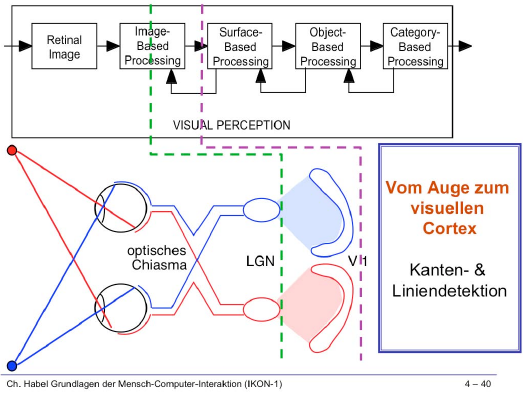
\includegraphics[width=0.7\textwidth]{eye-visual-cortex.png}
\end{center}

Durch verschiedene Verschaltung von rezeptiven Feldern ist es möglich, Kontrast-Kanten
zu erkennen. Ähnlich funktioniert computationelle Kantenerkennen. Der Kantenoperator
bildet die Differenz in der Intensitätsmatrix zweier benachbarter Zellen, entweder
horizontal oder vertikal (horizontaler Kantenoperator heißt, er erkennt horizontale
Kanten, wendet also auf vertikal benachbarte Zellen an). Im neuronalen Netzwerk ist
der Kantenoperator über exzitatorische und inhibitorische Verbindungen aufgebaut (Differenz).

Das Auge kann im \textbf{dreidimensionalen Farbraum} wahrnehmen. Der Farbraum hat dabei
die 3 Dimensionen Helligkeit (\emph{lightness}), Sättigung (\emph{saturation}) und
Farbton (\emph{hue}), wobei die letze Dimension zyklisch ist.

Nach intuitivem Farbempfinden gibt es 3 Paare komplementärer Farben: schwarz -- weiß,
rot -- grün und blau -- gelb.

Die ,,Luminanz'' einer Farbe beinhaltet nicht den Blauwert - daher ist von Details
mit konstanter Luminanz, etwa gelber Schrift auf einem Blau-Weiß-Verlauf, abzusehen
(Luminanz wird für Detailkontrast benötigt). Da außerdem die blauen Zapfen am geringsten
ausgeprägt sind, ist von blauem Text auf dunklem Hintergrund ebenfalls abzuraten.

\subsubsection{Tiefenwahrnehmung}

Wichtig für die Tiefenwahrnehmung sind die Distanz vom Objekt sowie die Ausrichtung
der Oberflächen (Vektor der Oberflächennormalen). Größere Objekte werden als ,,näher
dran'' empfunden. Dies kann zu Illusionen führen. Der Oberflächenvektor wird leicht
über den Lichteinfall und die resultierende Schattierung (\emph{shading}) erkannt.

\subsubsection{Objekterkennung}

Für die Objekterkennung wird das wahrgenommene Bild im Arbeitsgedächtnis mit bekannten
Objekten/Eindrücken aus dem Langzeitgedächtnis kombiniert.

\subsection{Das 2-Stufen-Modell der Wahrnehmung}

Wahrnehmung kann in 2 Stufen unterteilt werden. In der ersten Stufe wird parallel
und ohne Aufmerksamkeit (präattentiv, bottom-up) automatisch und schnell von Neuronenverbunden
verarbeitet. Die Information wird nur sehr kurz gespeichert. Im 2. Schritt wird
bewusst und zielgerichtet weiterverarbeitet, dies dauert länger und kann nicht
parallelisiert ablaufen (top-down).

Menschen können somit die Anzahl von Objekten im Sehfeld auch bei nur kurzer
Betrachtungsdauer (bis 400 ms) erkennen, ohne zählen zu müssen, wenn es sich um eine
kleine Anzahl Objekte handelt (3 - 8). Dieser Effekt heißt \textbf{subitizing}, und
ist im Gegensatz zum Zählen präattentiv. Ähnliche Phänomene sind \textbf{multiple object
tracking} (verfolge sich bewegende Objekte und indentifizieren hinterher die vorher
markierten) und \textbf{change blindness} (Dinge verändern sich, während die Aufmerksamkeit
auf andere Objekte gelenkt wird).

\subsection{Haptische Wahrnehmung}

... basiert auf Drucksensoren unter der Haut sowie kinesthethischen Rezeptoren in Muskeln,
Sehnen und Gelenken. Der haptische Sinn ist direkt, nur Objekte, mit denen Kontakt besteht,
können erfasst werden (Ausnahme: Hitzestrahlung).

Im Gegensatz zur visuellen Wahrnehmung ist die haptische Konturenerkennung von 2D-Objekten
sequentiell.
